\documentclass[11pt]{article}
\usepackage[margin=2.5cm]{geometry}
\usepackage{microtype}
\usepackage{amsmath,amssymb}
\usepackage{booktabs}
\usepackage{graphicx}
\usepackage{algorithm}
\usepackage{algpseudocode}
\usepackage{xcolor}
\usepackage[numbers,sort&compress]{natbib}
\usepackage[colorlinks=true,linkcolor=blue!50!black,citecolor=blue!50!black,urlcolor=blue!50!black]{hyperref}
\usepackage{url}
\setlength{\parskip}{0.4em}
\setlength{\emergencystretch}{3em}
\renewcommand{\arraystretch}{1.08}
% generated by paper/make_tables2.py
\newcommand{\accMainBalanced}{200}
\newcommand{\accMainBalancedRb}{80}
\newcommand{\accMainCap}{100}
\newcommand{\accMainNaive}{337}
\newcommand{\accMainSeedOnly}{0}
\newcommand{\accMainVerified}{20}
\newcommand{\accMainVerifiedMargin}{5}
\newcommand{\accNaiveBusiness}{2.5}
\newcommand{\accNaiveHealth}{48.8}
\newcommand{\accNaivePolitics}{44.1}
\newcommand{\accNaiveSports}{242.0}
\newcommand{\accRoundZeroCharlr}{0.870}
\newcommand{\accRoundZeroMlp}{0.845}
\newcommand{\agreeCharlr}{0.936}
\newcommand{\agreeMlp}{0.924}
\newcommand{\budFiveBalancedRb}{0.649}
\newcommand{\budFiveNaive}{0.621}
\newcommand{\budFiveSeedOnly}{0.649}
\newcommand{\budFiveVerified}{0.671}
\newcommand{\budFourZeroBalancedRb}{0.878}
\newcommand{\budFourZeroNaive}{0.859}
\newcommand{\budFourZeroSeedOnly}{0.879}
\newcommand{\budFourZeroVerified}{0.876}
\newcommand{\budOneZeroBalancedRb}{0.799}
\newcommand{\budOneZeroNaive}{0.800}
\newcommand{\budOneZeroSeedOnly}{0.797}
\newcommand{\budOneZeroVerified}{0.801}
\newcommand{\budTwoZeroBalancedRb}{0.852}
\newcommand{\budTwoZeroNaive}{0.697}
\newcommand{\budTwoZeroSeedOnly}{0.847}
\newcommand{\budTwoZeroVerified}{0.840}
\newcommand{\cmpBalancedRbVsVerified}{+0.010 [+0.002, +0.019]}
\newcommand{\cmpBalancedVsNaive}{+0.162 [+0.134, +0.191]}
\newcommand{\cmpCapVsNaive}{+0.125 [+0.093, +0.161]}
\newcommand{\cmpCharAgreeEffect}{+0.0014 [$-$0.0000, +0.0039]}
\newcommand{\cmpCharBalancedRb}{+0.002 [$-$0.003, +0.007]}
\newcommand{\cmpCharConfRb}{+0.017 [+0.007, +0.028]}
\newcommand{\cmpCharNaive}{+0.020 [+0.010, +0.030]}
\newcommand{\cmpCharVerified}{+0.019 [+0.009, +0.029]}
\newcommand{\cmpCharVerifiedThrZeroSeven}{+0.028 [+0.023, +0.033]}
\newcommand{\cmpCharVerifiedUncal}{$-$0.000 [$-$0.000, +0.000]}
\newcommand{\cmpCharVsMlp}{+0.026 [+0.021, +0.031]}
\newcommand{\cmpDevVerified}{+0.009 [+0.003, +0.016]}
\newcommand{\cmpMainBalanced}{+0.016 [+0.010, +0.020]}
\newcommand{\cmpMainBalancedRb}{+0.009 [+0.000, +0.018]}
\newcommand{\cmpMainCap}{$-$0.022 [$-$0.030, $-$0.013]}
\newcommand{\cmpMainNaive}{$-$0.147 [$-$0.177, $-$0.120]}
\newcommand{\cmpMainVerified}{$-$0.001 [$-$0.008, +0.004]}
\newcommand{\cmpMainVerifiedMargin}{$-$0.001 [$-$0.004, +0.001]}
\newcommand{\cwrongMlpBusiness}{0.4}
\newcommand{\cwrongMlpHealth}{0.1}
\newcommand{\cwrongMlpPolitics}{0.0}
\newcommand{\cwrongMlpSports}{0.0}
\newcommand{\devGainGtTwoSe}{0}
\newcommand{\devGainVerified}{+0.009}
\newcommand{\devSeVerified}{0.008}
\newcommand{\dsAFullLinear}{0.3}
\newcommand{\dsAFullMlp}{0.3}
\newcommand{\dsALowLinear}{0.3}
\newcommand{\dsALowMlp}{0.3}
\newcommand{\dsDeceFullLinear}{$-$0.019}
\newcommand{\dsDeceFullMlp}{$-$0.009}
\newcommand{\dsDeceLowLinear}{$-$0.037}
\newcommand{\dsDeceLowMlp}{+0.127}
\newcommand{\dsDiffFullLinear}{$-$0.001 [$-$0.003, +0.000]}
\newcommand{\dsDiffFullMlp}{+0.001 [$-$0.002, +0.004]}
\newcommand{\dsDiffLowLinear}{$-$0.014 [$-$0.019, $-$0.008]}
\newcommand{\dsDiffLowMlp}{$-$0.017 [$-$0.024, $-$0.010]}
\newcommand{\dsDistFullLinear}{0.899}
\newcommand{\dsDistFullMlp}{0.894}
\newcommand{\dsDistLowLinear}{0.817}
\newcommand{\dsDistLowMlp}{0.815}
\newcommand{\dsHardFullLinear}{0.901}
\newcommand{\dsHardFullMlp}{0.893}
\newcommand{\dsHardLowLinear}{0.831}
\newcommand{\dsHardLowMlp}{0.831}
\newcommand{\dsPFullLinear}{0.152}
\newcommand{\dsPFullMlp}{0.846}
\newcommand{\dsPLowLinear}{0.004}
\newcommand{\dsPLowMlp}{0.002}
\newcommand{\dsTFullLinear}{4}
\newcommand{\dsTFullMlp}{2}
\newcommand{\dsTLowLinear}{4}
\newcommand{\dsTLowMlp}{2}
\newcommand{\dsTeacherFullLinear}{0.909}
\newcommand{\dsTeacherFullMlp}{0.909}
\newcommand{\dsTeacherLowLinear}{0.843}
\newcommand{\dsTeacherLowMlp}{0.843}
\newcommand{\dsTostFullLinear}{$<$0.001}
\newcommand{\dsTostFullMlp}{$<$0.001}
\newcommand{\dsTostLowLinear}{0.893}
\newcommand{\dsTostLowMlp}{0.942}
\newcommand{\entMainBalanced}{1.386}
\newcommand{\entMainBalancedRb}{1.386}
\newcommand{\entMainCap}{0.959}
\newcommand{\entMainNaive}{0.624}
\newcommand{\entMainVerified}{0.971}
\newcommand{\entMainVerifiedMargin}{0.890}
\newcommand{\fCharBalancedRb}{0.872}
\newcommand{\fCharConfRb}{0.887}
\newcommand{\fCharNaive}{0.889}
\newcommand{\fCharNaiveMinusMlpNaive}{+0.192}
\newcommand{\fCharSeedOnly}{0.869}
\newcommand{\fCharVerified}{0.888}
\newcommand{\fCharVerifiedThrZeroSeven}{0.898}
\newcommand{\fCharVerifiedUncal}{0.869}
\newcommand{\fMainBalanced}{0.859}
\newcommand{\fMainBalancedRb}{0.852}
\newcommand{\fMainCap}{0.822}
\newcommand{\fMainNaive}{0.697}
\newcommand{\fMainSeedOnly}{0.843}
\newcommand{\fMainVerified}{0.842}
\newcommand{\fMainVerifiedMargin}{0.842}
\newcommand{\fwdSpeedup}{1.7}
\newcommand{\latSpeedup}{1.9}
\newcommand{\latStudent}{0.54}
\newcommand{\latTeacher}{1.01}
\newcommand{\meanConfCharlr}{0.858}
\newcommand{\meanConfMlp}{0.557}
\newcommand{\meanConfMlpBusiness}{0.491}
\newcommand{\meanConfMlpHealth}{0.551}
\newcommand{\meanConfMlpPolitics}{0.532}
\newcommand{\meanConfMlpSports}{0.602}
\newcommand{\mergedDistVsSeedHard}{$-$0.012 [$-$0.017, $-$0.007]}
\newcommand{\mergedGainStudentDev}{+0.002 [$-$0.000, +0.004]}
\newcommand{\mergedGainStudentTest}{+0.002 [$-$0.002, +0.005]}
\newcommand{\mergedGainTeacherDev}{+0.009 [+0.003, +0.016]}
\newcommand{\mergedGainTeacherTest}{$-$0.001 [$-$0.008, +0.004]}
\newcommand{\mergedN}{10}
\newcommand{\mergedPDistVsSeedHard}{0.006}
\newcommand{\mergedPStudentDev}{0.219}
\newcommand{\mergedPStudentTest}{0.562}
\newcommand{\mergedPTeacherDev}{0.031}
\newcommand{\mergedPTeacherTest}{0.844}
\newcommand{\mergedStudentFromFinal}{0.819}
\newcommand{\mergedStudentFromRoundZero}{0.817}
\newcommand{\mergedStudentHardPseudo}{0.829}
\newcommand{\mergedStudentSeedHard}{0.831}
\newcommand{\mergedStudentTaskTwoFullLabelsref}{0.899}
\newcommand{\mergedTeacherFinalLoop}{0.842}
\newcommand{\mergedTeacherFullLabelsref}{0.909}
\newcommand{\mergedTeacherRoundZero}{0.843}
\newcommand{\nSeeds}{10}
\newcommand{\nimpCharBalancedRb}{3/10}
\newcommand{\nimpCharConfRb}{7/10}
\newcommand{\nimpCharNaive}{9/10}
\newcommand{\nimpCharVerified}{7/10}
\newcommand{\nimpCharVerifiedThrZeroSeven}{10/10}
\newcommand{\nimpCharVerifiedUncal}{0/10}
\newcommand{\nimpMainBalanced}{10/10}
\newcommand{\nimpMainBalancedRb}{6/10}
\newcommand{\nimpMainCap}{1/10}
\newcommand{\nimpMainNaive}{0/10}
\newcommand{\nimpMainVerified}{3/10}
\newcommand{\nimpMainVerifiedMargin}{1/10}
\newcommand{\pBalancedRbVsVerified}{0.084}
\newcommand{\pBalancedVsNaive}{0.002}
\newcommand{\pCapVsNaive}{0.002}
\newcommand{\pCharAgreeEffect}{0.219}
\newcommand{\pCharBalancedRb}{0.562}
\newcommand{\pCharConfRb}{0.016}
\newcommand{\pCharNaive}{0.004}
\newcommand{\pCharVerified}{0.016}
\newcommand{\pCharVerifiedThrZeroSeven}{0.002}
\newcommand{\pCharVerifiedUncal}{0.500}
\newcommand{\pCharVsMlp}{0.002}
\newcommand{\pMainBalanced}{0.002}
\newcommand{\pMainBalancedRb}{0.164}
\newcommand{\pMainCap}{0.004}
\newcommand{\pMainNaive}{0.002}
\newcommand{\pMainVerified}{0.844}
\newcommand{\pMainVerifiedMargin}{0.750}
\newcommand{\phiCharlr}{0.768}
\newcommand{\phiMlp}{0.747}
\newcommand{\precMainBalanced}{0.979}
\newcommand{\precMainBalancedRb}{0.980}
\newcommand{\precMainCap}{0.987}
\newcommand{\precMainNaive}{0.984}
\newcommand{\precMainVerified}{0.971}
\newcommand{\precMainVerifiedMargin}{0.976}
\newcommand{\pvrCharlr}{0.135}
\newcommand{\pvrMlp}{0.280}
\newcommand{\recallMlpBusiness}{0.768}
\newcommand{\recallMlpHealth}{0.848}
\newcommand{\recallMlpPolitics}{0.866}
\newcommand{\recallMlpSports}{0.905}
\newcommand{\sdMainBalanced}{0.012}
\newcommand{\sdMainBalancedRb}{0.019}
\newcommand{\sdMainCap}{0.016}
\newcommand{\sdMainNaive}{0.048}
\newcommand{\sdMainSeedOnly}{0.013}
\newcommand{\sdMainVerified}{0.015}
\newcommand{\sdMainVerifiedMargin}{0.011}
\newcommand{\shareZeroNineMlpBusiness}{0.3}
\newcommand{\shareZeroNineMlpHealth}{2.3}
\newcommand{\shareZeroNineMlpPolitics}{0.8}
\newcommand{\shareZeroNineMlpSports}{4.4}
\newcommand{\testCiExclNaive}{10}
\newcommand{\testCiExclVerified}{0}
\newcommand{\thrZeroFiveNaive}{0.874}
\newcommand{\thrZeroFiveVerified}{0.891}
\newcommand{\thrZeroNineNaive}{0.697}
\newcommand{\thrZeroNineVerified}{0.840}
\newcommand{\thrZeroSevenNaive}{0.864}
\newcommand{\thrZeroSevenVerified}{0.846}
\newcommand{\tostMainVerified}{0.014}
\newcommand{\verCharDis}{207}
\newcommand{\verCharSel}{10366}
\newcommand{\verCharTeacherRight}{188}
\newcommand{\verCharVerRight}{19}
\newcommand{\verMainDis}{0}
\newcommand{\verMainSel}{983}
\newcommand{\verNaiveDis}{29}
\newcommand{\verNaiveSel}{3374}
\newcommand{\verThrDis}{1258}
\newcommand{\verThrRate}{10.5}
\newcommand{\verThrSel}{12035}
\newcommand{\verThrTeacherRight}{1013}
\newcommand{\verThrVerRight}{198}
\newcommand{\zeroNaiveBusiness}{5}
\newcommand{\zeroNaiveHealth}{0}
\newcommand{\zeroNaivePolitics}{0}
\newcommand{\zeroNaiveSports}{0}


\title{When High-Precision Pseudo-Labels Fail:\\
Class-Composition Bias in Low-Label Self-Training\\
for Amharic News Classification}
\author{Simachew Alamneh\\
\small Bonga University, Ethiopia \;\textbar\; iCog Labs AI Internship\\
\small \texttt{[corresponding author email]}}
\date{}

\begin{document}
\maketitle
\begin{abstract}
Self-training for low-resource text classification is usually guarded by a confidence threshold, a second-model check and a held-out roll-back. We test how well these guards work for Amharic news classification with only 80 labelled articles, using paired experiments over \nSeeds{} seeds on MasakhaNEWS. With a raw MLP teacher and a 0.9 confidence threshold, an unprotected loop loses \cmpMainNaive{} macro-F1 relative to the seed-only teacher on every seed, although \precMainNaive{} of its accepted pseudo-labels are correct. The teacher is underconfident, the threshold admits almost only sports and health articles (about 1\% of business articles against 78\% of sports articles), and the training set drifts. The failure is conditional: a calibrated character-level teacher or a lower threshold removes it, and class-balanced selection turns it into a consistent gain of \cmpMainBalanced{}. A feature-diverse second-model verifier rarely disagrees and is usually the one that is wrong when it does, because the two models' errors are strongly correlated; development-set roll-back prevents the collapse but cannot certify small gains. Distilling a teacher trained on all labels into a student with about 320 times fewer parameters left accuracy unchanged (equivalence within $\pm0.01$ macro-F1), while distilling from the low-label teacher reduced accuracy relative to training the student on the seed labels (\dsDiffLowLinear{} for a linear student). The loop's small development gain did not appear on the test set (\mergedGainTeacherTest{}). We release code, per-run results and seed-set indices.
\end{abstract}

\noindent\textbf{Keywords:} Amharic; self-training; pseudo-labelling; calibration; class imbalance; knowledge distillation; low-resource NLP


\section{Introduction}
Labelled data is the scarce resource in most African-language NLP. Unlabeled Amharic news text is easy to collect; hand-labelled articles are not. Self-training promises a way out: a model trained on a few labels predicts the rest, its most trustworthy predictions are added to the training set, and the process repeats. A standard safeguard is to keep only predictions that look reliable, for example those above a confidence threshold, perhaps confirmed by a second model, and to discard any round that hurts a held-out development set.

This paper asks how far such safeguards go in a realistic low-label setting, and it starts from a puzzling observation. In an initial three-seed study, a loop whose accepted pseudo-labels were 97 to 100\% correct still lost 0.11 to 0.17 macro-F1 on the test set. Per-item precision, the quantity most self-training work reports, was not warning us about anything. The question is why.

We follow that observation with a larger and more carefully controlled study (\nSeeds{} paired seeds, an explicit audit of the evaluation protocol, and interventions rather than only descriptions). Our answers are more nuanced than the initial result suggested.
\begin{enumerate}
\item \textbf{The failure is real but conditional.} With a raw MLP teacher and a 0.9 confidence threshold, the unprotected loop loses \cmpMainNaive{} macro-F1 (mean difference and 95\% bootstrap CI) relative to the seed-only teacher, on every seed, while pseudo-label precision stays at \precMainNaive{}. The accepted examples are heavily skewed towards one class: sports receives about 78\% of its pool articles as pseudo-labels, business about 1\%.
\item \textbf{The cause appears to be an underconfident teacher meeting a single global threshold.} The raw teacher is underconfident, most of all on business (mean confidence \meanConfMlpBusiness{} against recall \recallMlpBusiness{}), so a global threshold selects mostly the easiest class. A calibrated, stronger character-level teacher or a lower threshold removes the collapse, and class-balanced selection (top-$k$ per predicted class) turns it into a consistent gain of \cmpMainBalanced{}.
\item \textbf{The cross-representation verifier did almost nothing useful.} It rarely disagrees with the teacher, and when it does, it is usually the one that is wrong; teacher and verifier errors are strongly correlated.
\item \textbf{Development-set rollback is protective but noisy.} It prevents the collapse, but the development gain it reports is within sampling noise.
\end{enumerate}
We also examine knowledge distillation of the resulting teachers into small students, with linear and non-linear students and two supervision conditions. We do not claim methodological novelty; the contribution is a controlled, reproducible diagnosis and a simple remedy, evaluated with paired statistics.

\section{Related Work}
\paragraph{Self-training and pseudo-labelling.} Self-training has a long history in NLP \citep{yarowsky1995unsupervised} and was popularised for deep networks as pseudo-labelling \citep{lee2013pseudo}. Modern semi-supervised methods combine it with consistency regularisation, confidence thresholds and curricula \citep{sohn2020fixmatch,zhang2021flexmatch}, and with teacher--student iteration \citep{xie2020noisy}. Confirmation bias, in which early errors are reinforced in later rounds, is the central failure mode \citep{arazo2020pseudo}.

\paragraph{Selecting pseudo-labels.} Selection rules range from fixed confidence thresholds to uncertainty-aware filtering in language-model self-training \citep{wang2023upet}, decision-theoretic selection \citep{rodemann2023decision,rodemann2023likelihoods}, and conformal prediction sets with validity guarantees \citep{lienen2023conformal}. Our verifier, which requires agreement with a model built on a different feature view, represents the common practice of multi-view agreement; our experiments probe how much it adds.

\paragraph{Class imbalance in pseudo-labels.} Pseudo-labels can be class-skewed even when the labelled and unlabeled data are balanced. \citet{wang2022debiased} show that pseudo-labels produced by a classifier trained on balanced data are themselves heavily imbalanced, and propose debiasing; \citet{wei2021crest} rebalance self-training on genuinely imbalanced data and observe that minority classes yield high-precision pseudo-labels that standard selection under-uses. Our setting is balanced text classification with a tiny seed set; our finding is consistent with this literature and adds a text and low-resource data point, a calibration-based explanation, and a test of simple remedies.

\paragraph{Self-refinement and model collapse.} Test-time self-refinement changes outputs without changing weights \citep{madaan2023selfrefine}, while repeated training on model-generated data can degrade generative models \citep{shumailov2024collapse}. We study the weight-updating discriminative case, which is closer to classical self-training than to recursive self-improvement.

\paragraph{Calibration.} Neural classifiers are often miscalibrated, and temperature scaling is a simple, effective post-hoc fix \citep{guo2017calibration}. Calibration matters for self-training because confidence thresholds only mean the same thing across classes and rounds when confidence tracks correctness. Expected calibration error (ECE) measures the size of miscalibration but not its direction, so we also report mean confidence against accuracy.

\paragraph{Distillation.} We use the temperature-scaled soft-target loss of \citet{hinton2015distilling}.

\paragraph{Amharic and African-language news classification.} The Amharic dataset of \citet{azime2021amharic} and the Amharic portion of MasakhaNEWS \citep{adelani2023masakhanews} are the main resources for the task. MasakhaNEWS reports full-supervision baselines with African-centric encoders such as AfroXLMR \citep{alabi2022afroxlmr} and AfriBERTa \citep{ogueji2021afriberta}, and few-shot baselines such as pattern-exploiting training and SetFit \citep{schick2021pet,tunstall2022setfit}. Table~\ref{tab:ref} places our small models next to those published numbers.

\paragraph{Statistical practice.} For paired comparisons across runs we follow the guidance of \citet{dror2018hitchhiker}: paired tests, effect sizes with intervals, and no reliance on small differences in mean scores. To support ``no difference'' statements we use equivalence testing \citep{schuirmann1987comparison,lakens2017equivalence}, because a non-significant difference test does not show that an effect is absent.

\section{Problem Setting, Data and Protocol}
\paragraph{Data and licence.} We use the Amharic subset of MasakhaNEWS with its official splits: 1{,}311 training, 188 development and 376 test articles, four topics (business, health, politics, sports). Articles are crawled from BBC Amharic and annotated by five annotators (Fleiss' $\kappa=0.81$) \citep{adelani2023masakhanews}. The input is the headline followed by the body, truncated to 3{,}000 characters. The sources we found disagree on the licence: the dataset paper states release under an academic licence or CC BY-NC 4.0, whereas the Hugging Face dataset card lists AFL-3.0. We have not resolved this and ask readers to confirm the terms of use with the dataset authors; we redistribute no data.

\paragraph{Splits and labels.} For self-training we draw a stratified \emph{seed set} $S$ of $m$ labelled articles per class from the training split ($m=20$ unless stated, i.e.\ 80 labels). The remaining training articles form the \emph{unlabeled pool} $U$ (262 business, 330 health, 330 politics, 309 sports after removing a 20-per-class seed set). The pool's gold labels are used only to \emph{measure} pseudo-label quality and are never trained on. The development split decides roll-back, selects temperature and distillation hyper-parameters; the test split is used for final reporting.

\paragraph{Protocol audit.} Vectorisers (TF-IDF) are fitted on the text of the whole training split, including the unlabeled pool, without labels. Every model is trained from scratch in each round. Hyper-parameters were set once and not tuned per method. All experiments are paired by seed: the same seed set, initialisation and data order are used for every method within a seed. The initial three-seed study, whose test results we inspected, motivated the interventions studied here; the \nSeeds-seed suites and their comparisons were specified in code before they were run, but they are not formally preregistered, and we apply no multiple-comparison correction.

\paragraph{Metrics and statistics.} The main metric is macro-F1. ECE uses 15 equal-width confidence bins $(\ell, u]$ and skips empty bins. Pseudo-label precision is the fraction of accepted pseudo-labels that match the hidden gold label. The \emph{acceptance rate} of class $c$ is the number of accepted pseudo-labels of that class divided by the number of pool articles that truly belong to $c$. Class entropy is the natural-log entropy of the class distribution of the accepted set (maximum $\ln 4 = 1.386$). Paired differences are computed per seed. We report the mean difference with a bootstrap 95\% confidence interval over seeds (10{,}000 resamples), a two-sided Wilcoxon signed-rank test \citep{wilcoxon1945individual}, and, for ``no effect'' claims, a TOST equivalence test with margin $\pm0.01$ macro-F1. Within a seed we also bootstrap over test and development examples (1{,}000 resamples).

\section{Methods}
\subsection{Models and feature views}
The \emph{MLP teacher} is a two-layer network (256 hidden units, dropout 0.5; 30 epochs of Adam, learning rate $10^{-3}$, weight decay $10^{-4}$, batch size 32) on word 1--2-gram TF-IDF (10{,}000 features). The \emph{char-LR teacher} is a logistic regression ($C=100$) on character 2--4-gram TF-IDF (50{,}000 features). A \emph{cross-representation verifier} is a logistic regression ($C=10$) on the other view: character n-grams for the MLP teacher, word n-grams for the char-LR teacher. Both are fitted on the seed set only. The verifier shares the teacher's labels, so it is feature-diverse rather than statistically independent; Section~\ref{sec:verifier} measures how correlated their errors are.

\subsection{The self-training loop}
Let $f$ be the current teacher, $A$ the accepted pseudo-labelled examples (initially empty), $P=U\setminus A$ the remaining pool and $s$ the current development macro-F1. In round $r\le 5$ the teacher labels $P$, a selection rule picks candidates $C\subseteq P$, and a fresh model $f'$ is trained from scratch on $S\cup A\cup C$. With roll-back, $f'$ replaces $f$ if its development macro-F1 is at least $s$ plus a margin (zero unless stated; ties are accepted); then $A\leftarrow A\cup C$ and $s$ is updated. Otherwise $C$ is discarded and its articles stay in $P$, so they may be reconsidered later. Accepted pseudo-labels are never relabelled. The loop stops after two consecutive roll-backs. If no candidate is selected, $f'$ is retrained on $S\cup A$ with a different seed and the same acceptance rule applies. The \emph{naive} variant uses identical candidate generation but accepts every round.

\subsection{Selection rules}
\begin{itemize}
\item \textbf{Threshold:} accept predictions with confidence $\ge0.9$, optionally requiring the verifier to predict the same class.
\item \textbf{Cap:} the threshold rule, plus at most $k=10$ most-confident accepted examples per predicted class per round.
\item \textbf{Balanced:} for each predicted class, accept the $k=10$ most confident predictions among those with confidence $\ge0.5$, with no global threshold.
\end{itemize}
The balanced rule implicitly assumes classes are roughly balanced (a uniform per-class budget); we do not test imbalanced settings.

\subsection{Calibration}
Temperature scaling fits a single scalar $T$ minimising the negative log-likelihood of the development set, and divides the teacher's logits by $T$. For logistic regression the logits are the log-probabilities. The development set is therefore used both for calibration and for roll-back decisions.

\subsection{Distillation}
A student is trained with
\begin{equation}
\mathcal{L} \;=\; \alpha\,\mathrm{CE}(y,s) \;+\; (1-\alpha)\,T^{2}\,\mathrm{KL}\!\big(\mathrm{softmax}(t/T)\,\big\|\,\mathrm{softmax}(s/T)\big),
\label{eq:kd}
\end{equation}
with teacher logits $t$, student logits $s$, temperature $T$ and mixing weight $\alpha$. Rows without a hard label contribute only to the KL term. We sweep $T\in\{1,2,4\}$ and $\alpha\in\{0.3,0.5,0.7\}$ and select the pair with the best mean development macro-F1, separately for each condition and student family. Students are either linear or a small MLP (64 hidden units) on a 2{,}000-feature unigram TF-IDF view.

\section{System Architecture}
Figure~\ref{fig:arch} shows the merged architecture implemented in the accompanying code. \emph{Recursive learning} (left): a teacher trained on the 80 seed labels pseudo-labels the unlabeled pool, only verified predictions are admitted, and a fresh copy of the teacher is retrained on the seed set plus the accepted pseudo-labels. \emph{Knowledge distillation} (centre): the resulting teacher supplies soft targets that, together with gold labels, train a small student under the combined loss of Equation~\eqref{eq:kd}. \emph{Evaluation and safeguards} (right): a development-set gate accepts or rolls back each round, gold labels of the pool are used only for monitoring, and the test split is read once at the end. The same components also run on their own: the left pillar alone is the self-training experiment (Task~1), the centre pillar with a full-label teacher is the distillation experiment (Task~2), and the whole pipeline is the merged experiment (Task~3). Detailed flowcharts and an entity-relationship diagram are in the repository (\texttt{docs/}).

\begin{figure}[t]
\centering
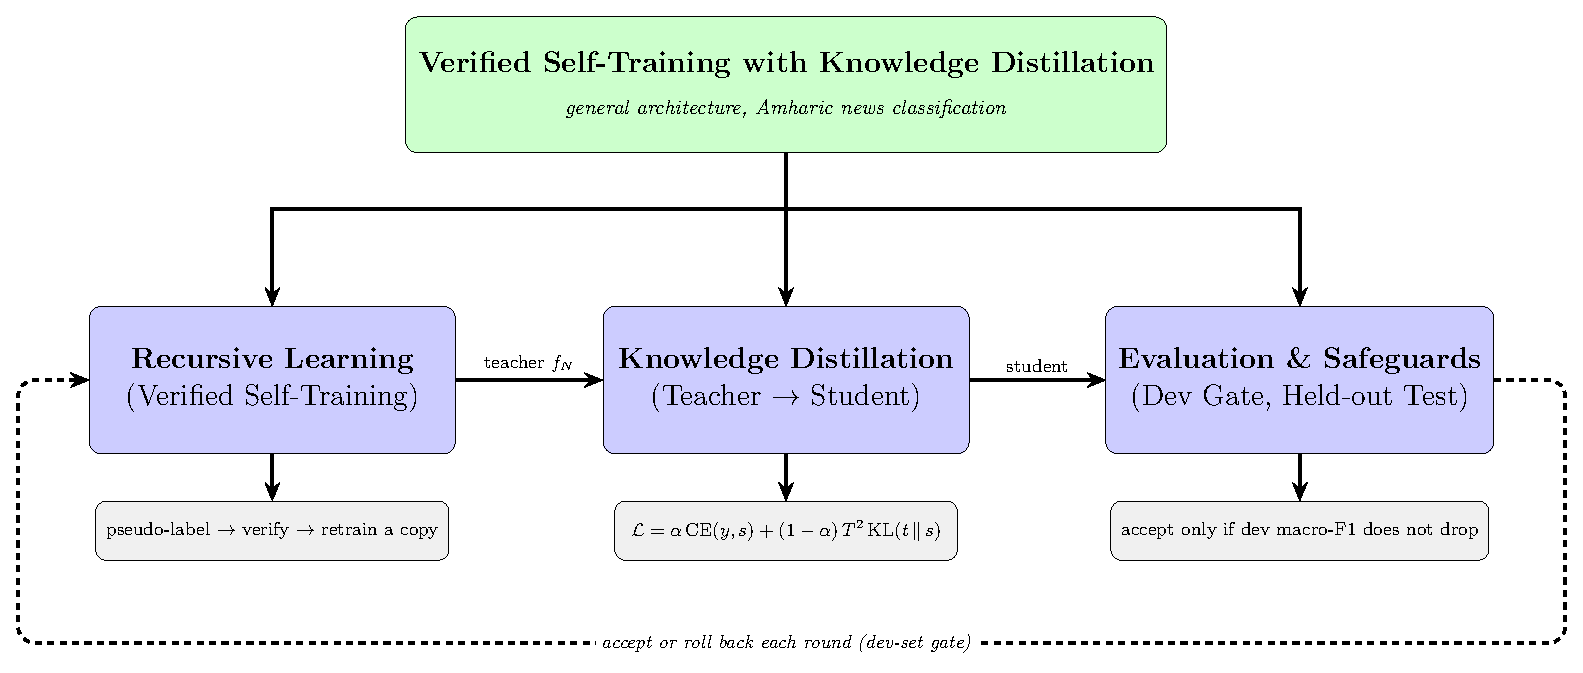
\includegraphics[width=\textwidth]{../docs/abstract/merged_overview.pdf}
\caption{Merged architecture: verified self-training (left), knowledge distillation (centre) and evaluation safeguards (right). The dashed arrow shows the development-set gate that accepts or rolls back each round.}\label{fig:arch}
\end{figure}

\section{Results}
All results are test macro-F1 (mean $\pm$ s.d.\ over \nSeeds{} paired seeds) unless stated; ``$\Delta$'' is the paired difference to the seed-only teacher with its 95\% bootstrap CI.

\subsection{Baselines and published reference points}
At 20 labels per class the seed-only MLP teacher scores \fMainSeedOnly{} and the seed-only char-LR scores \fCharSeedOnly{}; the char-LR is better on every seed (paired difference \cmpCharVsMlp{}, Wilcoxon $p$ = \pCharVsMlp). Table~\ref{tab:ref} lists published Amharic results from the MasakhaNEWS paper. They use weighted F1, pretrained encoders and, for few-shot methods, different draws of labelled examples, so they are reference points rather than comparisons. They indicate that our TF-IDF models are well below what encoders and few-shot methods reach at the same label budget, which is an important limit on how far our conclusions about self-training can be generalised.

\begin{table}[t]
\centering\small
\caption{Published Amharic MasakhaNEWS results (weighted F1, \citealp{adelani2023masakhanews}), shown for orientation only. ``$k$ shots'' means $k$ labelled articles per class.}\label{tab:ref}
\begin{tabular}{lccccc}
\toprule
Method & 10 shots & 20 shots & 50 shots & Full training set \\
\midrule
PET (AfroXLMR-large) & 91.1 & 92.7 & 92.9 & -- \\
Fine-tuned AfroXLMR-large & 75.5 & 88.5 & 91.4 & 94.4 \\
Fine-tuned LaBSE & 79.0 & 90.3 & 89.6 & 92.5 \\
SetFit (LaBSE) & 84.8 & 87.9 & 88.6 & -- \\
Fine-tuned AfroXLMR-base & -- & -- & -- & 94.2 \\
Count-vector MLP & -- & -- & -- & 92.0 \\
\bottomrule
\end{tabular}
\end{table}

\subsection{Self-training with the MLP teacher}
Table~\ref{tab:main} gives the central comparison. The verified loop (confidence, agreement, roll-back) is statistically indistinguishable from doing nothing: $\Delta$ = \cmpMainVerified (Wilcoxon $p$ = \pMainVerified) and the equivalence test supports a true effect within $\pm0.01$ ($p$ = \tostMainVerified). The loop accepted only about \accMainVerified{} pseudo-labels on average. Without roll-back the loop is clearly harmful: $\Delta$ = \cmpMainNaive, improving on \nimpMainNaive{} seeds (Wilcoxon $p$ = \pMainNaive), even though the precision of the accepted set is \precMainNaive.

\begin{table}[t]
\centering\small
\caption{MLP teacher, 20 labels per class, \nSeeds{} paired seeds. PL precision = precision of accepted pseudo-labels against hidden gold labels. ``Accepted'' = mean size of the accepted set.}\label{tab:main}
\resizebox{\textwidth}{!}{\begin{tabular}{lccccc}
\toprule
Variant & Test macro-F1 & $\Delta$ vs seed-only [95\% CI] & Wilcoxon $p$ & Accepted & PL precision \\
\midrule
Seed-only teacher (no loop) & 0.843\,$\pm$\,0.013 & -- & -- & 0 & -- \\
\addlinespace
Verified loop (confidence + agreement + rollback) & 0.842\,$\pm$\,0.015 & $-$0.001 [$-$0.008, +0.004] & 0.844 & 20 & 0.971 \\
Verified loop, acceptance margin 0.01 & 0.842\,$\pm$\,0.011 & $-$0.001 [$-$0.004, +0.001] & 0.750 & 5 & 0.976 \\
Naive loop (confidence, no rollback) & 0.697\,$\pm$\,0.048 & $-$0.147 [$-$0.177, $-$0.120] & 0.002 & 337 & 0.984 \\
Per-class cap (10 per class per round), no rollback & 0.822\,$\pm$\,0.016 & $-$0.022 [$-$0.030, $-$0.013] & 0.004 & 100 & 0.987 \\
Balanced top-$k$ per class, no rollback & 0.859\,$\pm$\,0.012 & +0.016 [+0.010, +0.020] & 0.002 & 200 & 0.979 \\
Balanced top-$k$ per class + rollback & 0.852\,$\pm$\,0.019 & +0.009 [+0.000, +0.018] & 0.164 & 80 & 0.980 \\
\bottomrule
\end{tabular}
}
\end{table}

\subsection{Why the unprotected loop collapses}
Table~\ref{tab:classes} shows what the loops accepted. The naive loop accepts on average \accNaiveSports{} sports, \accNaiveHealth{} health, \accNaivePolitics{} politics and \accNaiveBusiness{} business articles, i.e.\ roughly 1\% of the business pool against 78\% of the sports pool. Precision is high because the accepted articles are the easy ones; the training set they create is nonetheless unrepresentative, and the teacher retrained on it drifts towards the over-represented class.

\begin{table}[t]
\centering\small
\caption{Accepted pseudo-labels per class at the end of the loop (mean over seeds; acceptance rate $=$ accepted / pool size of that class in parentheses).}\label{tab:classes}
\resizebox{\textwidth}{!}{\begin{tabular}{lcccc}
\toprule
Variant & Business & Health & Politics & Sports \\
\midrule
Naive loop (confidence, no rollback) & 2.5 (1.0\%) & 48.8 (14.8\%) & 44.1 (13.4\%) & 242.0 (78.3\%) \\
Per-class cap (10 per class per round), no rollback & 2.4 (0.9\%) & 25.9 (7.8\%) & 22.5 (6.8\%) & 48.7 (15.8\%) \\
Balanced top-$k$ per class, no rollback & 50.0 (19.1\%) & 50.0 (15.2\%) & 50.0 (15.2\%) & 50.0 (16.2\%) \\
Verified loop (confidence + agreement + rollback) & 0.3 (0.1\%) & 5.2 (1.6\%) & 3.2 (1.0\%) & 11.5 (3.7\%) \\
\bottomrule
\end{tabular}
}
\end{table}

Table~\ref{tab:diag} shows why. The raw MLP teacher is strongly underconfident: its mean confidence is only \meanConfMlp{} against accuracy \accRoundZeroMlp{} on test, and the share of pool articles above 0.9 confidence is \shareZeroNineMlpSports\% for sports but \shareZeroNineMlpBusiness\% for business. Business also has the lowest recall (\recallMlpBusiness) and the lowest mean confidence (\meanConfMlpBusiness), while ``confidently wrong'' business predictions are rare (\cwrongMlpBusiness{} per seed on average). So the conjecture from our earlier study is supported: business is not mislabelled with high confidence, it simply almost never reaches the threshold. The confusion matrix in the appendix shows business articles are mostly confused with health and politics. With a single global threshold, a teacher in this regime selects almost exclusively the class it is most confident about.

\begin{table}[t]
\centering\small
\caption{Round-0 confidence diagnostics on the unlabeled pool (mean over seeds): mean and median confidence per true class, share above the 0.9 threshold, confidently wrong predictions (count per seed) and recall. The calibrated char-LR is shown for contrast.}\label{tab:diag}
\resizebox{\textwidth}{!}{\begin{tabular}{llcccccc}
\toprule
Teacher & Class & Pool & Mean conf. & Median conf. & Conf.\ $\ge$ 0.9 (\%) & Confidently wrong & Recall \\
\midrule
MLP (raw) & Business & 262 & 0.491 & 0.466 & 0.3 & 0.4 & 0.768 \\
 & Health & 330 & 0.551 & 0.539 & 2.3 & 0.1 & 0.848 \\
 & Politics & 330 & 0.532 & 0.512 & 0.8 & 0.0 & 0.866 \\
 & Sports & 309 & 0.602 & 0.601 & 4.4 & 0.0 & 0.905 \\
\addlinespace
Char-LR (calibrated) & Business & 262 & 0.803 & 0.856 & 42.9 & 10.3 & 0.806 \\
 & Health & 330 & 0.866 & 0.957 & 62.5 & 4.1 & 0.872 \\
 & Politics & 330 & 0.848 & 0.921 & 55.8 & 6.0 & 0.881 \\
 & Sports & 309 & 0.898 & 0.978 & 71.9 & 2.0 & 0.918 \\
\bottomrule
\end{tabular}
}
\end{table}

\subsection{Class-aware selection}
Table~\ref{tab:main} also reports two interventions that do not touch the teacher. A per-class cap alone is not enough: it reduces the damage (\cmpCapVsNaive{} relative to the naive loop) but still ends below the seed-only teacher ($\Delta$ = \cmpMainCap), because it only limits the dominant class and does nothing for the starved one. Balanced top-$k$ selection, which forces every class into every round, removes the collapse and gives a consistent gain: $\Delta$ = \cmpMainBalanced, improved on \nimpMainBalanced{} seeds, Wilcoxon $p$ = \pMainBalanced, with precision \precMainBalanced{} and maximal class entropy (Table~\ref{tab:classes}). Adding roll-back to balanced selection shrinks the gain to $\Delta$ = \cmpMainBalancedRb ($p$ = \pMainBalancedRb): the development set rejects some rounds that were in fact helpful. Class composition of the accepted set is therefore a causal ingredient of the failure and not just a correlate, at least in this setting.

\subsection{The verifier}\label{sec:verifier}
Table~\ref{tab:verifier} reports how often the verifier disagrees with a teacher prediction that passed the selection rule, and who is right when it does. For the verified MLP loop it never disagreed (\verMainDis{} of \verMainSel{} selected pseudo-labels); even in the naive loop, which selects many more articles, it disagreed on \verNaiveDis{} of \verNaiveSel{}. With the char-LR teacher the verifier disagrees more often (\verCharDis{} of \verCharSel{}), but the teacher was right in \verCharTeacherRight{} of those cases and the verifier in \verCharVerRight. At a lower threshold of 0.7, it vetoes \verThrDis{} of \verThrSel{} candidates (\verThrRate\%), and in \verThrTeacherRight{} of them the vetoed teacher label was correct against \verThrVerRight{} where the verifier was. The reason is visible in Table~\ref{tab:vercorr}: teacher and verifier errors are strongly correlated (error correlation $\phi$ = \phiMlp for MLP versus char-LR and $\phi$ = \phiCharlr for char-LR versus word-LR), and when the teacher is wrong the verifier is right only \pvrMlp{} (respectively \pvrCharlr) of the time. A second view built from the same few labels shares the first view's blind spots, so ``agreement'' filters out little and ``disagreement'' mostly removes correct pseudo-labels. Direct effect on accuracy: verified minus confidence-plus-roll-back for the char-LR teacher is \cmpCharAgreeEffect{} ($p$ = \pCharAgreeEffect).

\begin{table}[t]
\centering\small
\caption{Verifier activity: candidates that passed the selection rule, disagreements with the verifier, and who was correct on the disagreements (counts summed over seeds).}\label{tab:verifier}
\begin{tabular}{llrrrrr}
\toprule
Teacher & Variant & Selected & Disagreements & Rate (\%) & Teacher right & Verifier right \\
\midrule
MLP & naive & 3374 & 29 & 0.9 & 25 & 4 \\
MLP & verified & 983 & 0 & 0.0 & 0 & 0 \\
Char-LR & naive & 8685 & 130 & 1.5 & 117 & 13 \\
Char-LR & confidence + rollback & 10396 & 98 & 0.9 & 86 & 12 \\
Char-LR & verified & 10366 & 207 & 2.0 & 188 & 19 \\
Char-LR & verified, thr.\ 0.7 & 12035 & 1258 & 10.5 & 1013 & 198 \\
\bottomrule
\end{tabular}

\end{table}
\begin{table}[t]
\centering\small
\caption{Error dependence between teacher and verifier on the test set (mean over seeds).}\label{tab:vercorr}
\resizebox{\textwidth}{!}{\begin{tabular}{lcccccc}
\toprule
Teacher & Agreement & Teacher acc. & Verifier acc. & Error $\phi$ & P(both wrong) & P(ver.\ right $|$ teacher wrong) \\
\midrule
MLP vs char-LR & 0.924 & 0.845 & 0.869 & 0.747 & 0.112 & 0.280 \\
Char-LR vs word-LR & 0.936 & 0.870 & 0.848 & 0.768 & 0.112 & 0.135 \\
\bottomrule
\end{tabular}
}
\end{table}

\subsection{A stronger, calibrated teacher}
Table~\ref{tab:charlr} repeats the loop with a char-LR teacher whose confidence is temperature-scaled on the development set. The picture changes. There is no collapse: even the naive loop improves ($\Delta$ = \cmpCharNaive, $p$ = \pCharNaive), and the verified loop gains $\Delta$ = \cmpCharVerified (improved on \nimpCharVerified{} seeds, $p$ = \pCharVerified). Agreement and roll-back add essentially nothing over confidence alone. Lowering the threshold to 0.7 gives the best result, $\Delta$ = \cmpCharVerifiedThrZeroSeven (\nimpCharVerifiedThrZeroSeven{} seeds). Without calibration, almost nothing passes the 0.9 threshold and the loop does nothing ($\Delta$ = \cmpCharVerifiedUncal), which re-states the role of calibration. Balanced selection with roll-back does not help this teacher ($\Delta$ = \cmpCharBalancedRb, $p$ = \pCharBalancedRb).

\begin{table}[t]
\centering\small
\caption{Char-LR teacher with temperature-scaled confidence, 20 labels per class, \nSeeds{} paired seeds.}\label{tab:charlr}
\resizebox{\textwidth}{!}{\begin{tabular}{lccccc}
\toprule
Variant & Test macro-F1 & $\Delta$ vs seed-only [95\% CI] & Wilcoxon $p$ & Accepted & PL precision \\
\midrule
Seed-only char-LR (calibrated) & 0.869\,$\pm$\,0.016 & -- & -- & 0 & -- \\
\addlinespace
Naive (no rollback) & 0.889\,$\pm$\,0.014 & +0.020 [+0.010, +0.030] & 0.004 & 868 & 0.966 \\
Confidence + rollback & 0.887\,$\pm$\,0.014 & +0.017 [+0.007, +0.028] & 0.016 & 613 & 0.970 \\
Verified (agreement + rollback) & 0.888\,$\pm$\,0.013 & +0.019 [+0.009, +0.029] & 0.016 & 629 & 0.970 \\
Verified, threshold 0.7 & 0.898\,$\pm$\,0.009 & +0.028 [+0.023, +0.033] & 0.002 & 1019 & 0.939 \\
Verified, uncalibrated confidence & 0.869\,$\pm$\,0.016 & $-$0.000 [$-$0.000, +0.000] & 0.500 & 15 & 0.978 \\
Balanced top-$k$ + rollback & 0.872\,$\pm$\,0.016 & +0.002 [$-$0.003, +0.007] & 0.562 & 68 & 0.972 \\
\bottomrule
\end{tabular}
}
\end{table}

\subsection{Development-set optimism, thresholds and label budgets}
\paragraph{Development optimism.} The verified MLP loop improves the development macro-F1 by \devGainVerified{} on average (paired CI \cmpDevVerified), against a bootstrap standard error of the development estimate of \devSeVerified{} on 188 articles; in \devGainGtTwoSe{} of \nSeeds{} seeds does the gain exceed two standard errors, and in \testCiExclVerified{} of \nSeeds{} seeds does the within-seed test-bootstrap interval of the change exclude zero (for the naive loop: \testCiExclNaive{}). Roll-back on 188 articles is thus a coarse instrument: it catches the large collapse but cannot certify small gains. An acceptance margin of 0.01 changed nothing measurable ($\Delta$ = \cmpMainVerifiedMargin).

\paragraph{Threshold sensitivity.} Table~\ref{tab:thr} shows that part of the MLP collapse is a threshold artefact: with the unprotected loop at thresholds 0.5 and 0.7 the loop improves (\thrZeroFiveNaive{} and \thrZeroSevenNaive{} against \thrZeroNineNaive{} at 0.9), because enough articles from every class pass. Confidence thresholds therefore need to be chosen with the class composition of the accepted set in mind, not only the precision.

\paragraph{Label budget.} Table~\ref{tab:budget} varies the labels per class (five seeds). The seed-only teacher improves quickly with more labels. The naive loop is the least reliable variant, with by far its largest loss at 20 labels per class; at 10 labels per class it matches the other variants. We do not have an explanation beyond the interaction between teacher confidence and the fixed threshold.

\begin{table}[t]
\centering\small
\caption{MLP teacher, naive and verified loops at confidence thresholds 0.5, 0.7 and 0.9 (five seeds; $\Delta$ relative to the seed-only teacher of the same seeds).}\label{tab:thr}
\resizebox{\textwidth}{!}{\begin{tabular}{lccccc}
\toprule
Threshold & Variant & Test macro-F1 & $\Delta$ vs seed-only & Accepted & PL precision \\
\midrule
0.5 & naive & 0.874\,$\pm$\,0.014 & +0.028 & 1210 & 0.896 \\
0.5 & verified & 0.891\,$\pm$\,0.017 & +0.045 & 950 & 0.942 \\
0.7 & naive & 0.864\,$\pm$\,0.024 & +0.018 & 1091 & 0.916 \\
0.7 & verified & 0.846\,$\pm$\,0.018 & $-$0.000 & 336 & 0.981 \\
0.9 & naive & 0.697\,$\pm$\,0.056 & $-$0.150 & 326 & 0.986 \\
0.9 & verified & 0.840\,$\pm$\,0.016 & $-$0.007 & 30 & 0.975 \\
\bottomrule
\end{tabular}
}
\end{table}
\begin{table}[t]
\centering\small
\caption{Test macro-F1 by label budget (MLP teacher, threshold 0.9, five seeds).}\label{tab:budget}
\resizebox{\textwidth}{!}{\begin{tabular}{lcccc}
\toprule
Labels per class (total) & Seed-only & Verified & Naive & Balanced + rollback \\
\midrule
5 (20) & 0.649\,$\pm$\,0.071 & 0.671\,$\pm$\,0.064 & 0.621\,$\pm$\,0.111 & 0.649\,$\pm$\,0.071 \\
10 (40) & 0.797\,$\pm$\,0.024 & 0.801\,$\pm$\,0.025 & 0.800\,$\pm$\,0.025 & 0.799\,$\pm$\,0.044 \\
20 (80) & 0.847\,$\pm$\,0.014 & 0.840\,$\pm$\,0.016 & 0.697\,$\pm$\,0.056 & 0.852\,$\pm$\,0.018 \\
40 (160) & 0.879\,$\pm$\,0.008 & 0.876\,$\pm$\,0.014 & 0.859\,$\pm$\,0.027 & 0.878\,$\pm$\,0.013 \\
\bottomrule
\end{tabular}
}
\end{table}

\subsection{Distillation: compression, not accuracy}\label{sec:distill}
Table~\ref{tab:dist} separates two supervision conditions that the earlier study mixed. In the \emph{full-label} condition the teacher is trained on all 1{,}311 gold labels and the student sees all training inputs with gold labels (teacher macro-F1 \dsTeacherFullLinear). Soft targets change accuracy by \dsDiffFullLinear{} for a linear student (Wilcoxon $p$ = \dsPFullLinear) and \dsDiffFullMlp{} for an MLP student ($p$ = \dsPFullMlp); both are equivalent to hard-label training within $\pm0.01$ (TOST $p<0.001$). Soft targets did lower the calibration error (\dsDeceFullLinear{} and \dsDeceFullMlp{} ECE respectively). In the \emph{low-label} condition the teacher is trained on the 80 seed labels, and the student sees seed and pool inputs with hard labels on the seed set only. Here soft targets \emph{hurt}: \dsDiffLowLinear{} for the linear student ($p$ = \dsPLowLinear) and \dsDiffLowMlp{} for the MLP student ($p$ = \dsPLowMlp), relative to a student trained on the seed labels alone. A teacher with macro-F1 \dsTeacherLowLinear{} passes on its own errors, and the student has no other source of information. The extension used a reduced $(T,\alpha)$ grid ($T\in\{2,4\}$, $\alpha\in\{0.3,0.7\}$), selected on development data; the earlier three-seed sweep over a $3\times3$ grid also found no accuracy gain.

\begin{table}[t]
\centering\small
\caption{Distillation extension (\nSeeds{} paired seeds): student macro-F1 with hard labels versus the dev-selected distilled student, paired difference with 95\% CI, Wilcoxon $p$, and change in ECE. ``All gold labels'': teacher and student see all training labels. ``80 labels'': teacher trained on the seed set; students see seed and pool inputs, hard labels only on the seed set.}\label{tab:dist}
\resizebox{\textwidth}{!}{\begin{tabular}{llcccccc}
\toprule
Condition & Student & $(T,\alpha)$ & Hard F1 & Distilled F1 & $\Delta$ [95\% CI] & Wilcoxon $p$ & $\Delta$ECE \\
\midrule
All gold labels & Linear & (4, 0.3) & 0.901 & 0.899 & $-$0.001 [$-$0.003, +0.000] & 0.152 & $-$0.019 \\
All gold labels & MLP (64) & (2, 0.3) & 0.893 & 0.894 & +0.001 [$-$0.002, +0.004] & 0.846 & $-$0.009 \\
80 labels & Linear & (4, 0.3) & 0.831 & 0.817 & $-$0.014 [$-$0.019, $-$0.008] & 0.004 & $-$0.037 \\
80 labels & MLP (64) & (2, 0.3) & 0.831 & 0.815 & $-$0.017 [$-$0.024, $-$0.010] & 0.002 & +0.127 \\
\bottomrule
\end{tabular}
}
\end{table}

\paragraph{Compression.} The linear student has 8{,}004 parameters against 2{,}561{,}284 for the MLP teacher (about 320 times fewer) and a serialised size of 33~KB against about 10~MB. Measured as a forward pass on precomputed features, the student is about 3.4 times faster (Task~2); including vectorisation and sparse-tensor construction for a single article, the end-to-end speed-up is only \latSpeedup{} times (Table~\ref{tab:lat}: \latTeacher{} ms against \latStudent{} ms), because TF-IDF extraction does not shrink with the model. The cost in accuracy is about 0.7 to 0.9 macro-F1 points relative to the full-label teacher.

\begin{table}[t]
\centering\small
\caption{Single-article latency on one CPU thread (median over 200 test articles).}\label{tab:lat}
\begin{tabular}{lccc}
\toprule
Model & Vectorise (ms) & Forward (ms) & End-to-end (ms) \\
\midrule
Teacher & 0.635 & 0.310 & 1.012 \\
Student & 0.356 & 0.178 & 0.543 \\
\bottomrule
\end{tabular}

\end{table}

\subsection{The merged pipeline}
Table~\ref{tab:t3} gives the merged results over \mergedN{} seeds. The loop's teacher improves on the development set (\mergedGainTeacherDev{}, Wilcoxon $p$ = \mergedPTeacherDev) but not on the test set (\mergedGainTeacherTest{}, $p$ = \mergedPTeacherTest): the development gain is a selection effect, not an improvement that generalises. Accordingly there is no gain for distillation to preserve: students distilled from the loop's teacher and from the round-0 teacher differ by \mergedGainStudentTest{} on test ($p$ = \mergedPStudentTest). Both distilled students are below a student trained on the seed labels alone (\mergedDistVsSeedHard{} for the loop's student, $p$ = \mergedPDistVsSeedHard), consistent with Section~\ref{sec:distill}.

\begin{table}[t]
\centering\small
\caption{Merged pipeline, \mergedN{} paired seeds. ``(ref.)'' rows use all gold labels and are upper references, not comparable under the same label budget.}\label{tab:t3}
\begin{tabular}{lcc}
\toprule
Model & Test macro-F1 & Test ECE \\
\midrule
Teacher, round 0 & 0.843\,$\pm$\,0.013 & 0.289\,$\pm$\,0.011 \\
Teacher, after loop & 0.842\,$\pm$\,0.015 & 0.266\,$\pm$\,0.025 \\
\addlinespace
Student, hard labels (seed set) & 0.831\,$\pm$\,0.013 & 0.288\,$\pm$\,0.010 \\
Student, hard labels (seed + accepted) & 0.829\,$\pm$\,0.012 & 0.267\,$\pm$\,0.022 \\
Student, distilled from round-0 teacher & 0.817\,$\pm$\,0.016 & 0.251\,$\pm$\,0.014 \\
Student, distilled from loop teacher & 0.819\,$\pm$\,0.016 & 0.231\,$\pm$\,0.017 \\
\addlinespace
Student, distilled, full-label teacher (ref.) & 0.899\,$\pm$\,0.002 & 0.045\,$\pm$\,0.004 \\
Teacher, all gold labels (ref.) & 0.909\,$\pm$\,0.003 & 0.029\,$\pm$\,0.006 \\
\bottomrule
\end{tabular}

\end{table}

\section{Discussion}
\paragraph{Per-item precision is not enough; composition and calibration matter.} A pseudo-label set can be nearly perfectly accurate and still be a bad training set. In our setting the cause appears to be a confidence threshold applied to an underconfident, class-uneven teacher. Using a calibrated, stronger teacher or a lower threshold removed the collapse, and forcing balanced per-class selection turned it into a consistent gain. We did not isolate calibration for the MLP teacher itself (temperature scaling was applied only to the char-LR teacher), so the role of calibration there rests on the diagnostics in Table~\ref{tab:diag} and the threshold study. We therefore recommend that self-training studies report per-class acceptance rates and the class entropy of the accepted set alongside precision, and that they calibrate confidence before thresholding it. The balanced rule assumes a roughly uniform class prior; for imbalanced data a prior estimate or a rebalancing method \citep{wei2021crest,wang2022debiased} is needed.

\paragraph{A feature-diverse verifier is not an independent one.} Our verifier shares the teacher's few labels; its errors correlate strongly with the teacher's, so agreement is weak evidence and disagreement is more often the verifier's mistake. A verifier that adds information would need different supervision or different data, for example a pretrained encoder, rather than another view of the same eighty labels.

\paragraph{Roll-back is protective, not diagnostic.} It stops the large collapse, but with 188 development articles it cannot separate small gains from noise. The loop's development gain was statistically detectable across seeds while its test change was not, which is the signature of selection on a small set. Reporting both, with intervals, makes this visible.

\paragraph{Distillation helps size, not accuracy, and cannot repair a weak teacher.} With a strong teacher, distillation preserved accuracy and improved calibration; with the low-label teacher it reduced accuracy. The speed-up depends on where latency is measured.

\section{Limitations}
\begin{itemize}
\item \textbf{Feature-based models.} All models use TF-IDF features, so that everything runs on a CPU. Published encoder and few-shot results on the same dataset are much stronger (Table~\ref{tab:ref}); we did not run AfroXLMR or AfriBERTa teachers, and our conclusions may differ with them.
\item \textbf{One dataset, one language, four classes.} Paired seeds quantify seed-set and initialisation variance, not variation across datasets or languages. The collapse we diagnose depends on the teacher and the threshold (Tables~\ref{tab:charlr}, \ref{tab:thr}).
\item \textbf{Development set used twice.} It serves for calibration and for roll-back (and for selecting distillation hyper-parameters); a separate acceptance split would avoid this.
\item \textbf{Calibration of the MLP teacher was not tested in isolation}, and balanced selection assumes balanced classes and was not tested on imbalanced data. Its budget $k$ and floor were fixed once and not tuned.
\item \textbf{Exploratory origins and multiple comparisons.} The interventions were suggested by an initial three-seed study whose test results we inspected; we report many paired tests without correction and the 95\% intervals should be read as descriptive.
\item \textbf{Reduced grids.} The distillation extension used a $2\times2$ $(T,\alpha)$ grid; label-budget and threshold studies used five seeds.
\item \textbf{Hardware-dependent latency.} Measurements are single-thread CPU timings on one machine.
\item \textbf{Licence.} Licensing information for the dataset is inconsistent across sources (Section~3); we redistribute no data.
\end{itemize}

\section{Conclusion}
In a low-label Amharic news setting, a high-precision pseudo-label set from a confidence-thresholded loop can still collapse a teacher, because the set is class-skewed. The failure comes from an underconfident teacher meeting a single global threshold; it disappears with a calibrated, stronger teacher, a lower threshold or class-balanced selection, and the latter gives a small but consistent gain. A second-view verifier built from the same labels contributes almost nothing, development-set roll-back protects against collapse without certifying gains, and distillation compresses a strong teacher without changing accuracy but cannot rescue a weak one. The most useful next steps are encoder-based teachers, a comparison across MasakhaNEWS languages, imbalanced class priors, and conformal or uncertainty-based selection.

\section*{Reproducibility}
{\sloppy Code, configurations, seed-set indices (\texttt{results/research/seed\_sets.json}), per-run results and table generators are at \url{https://github.com/simachewalamneh/amharic-verified-self-improvement}. Tables and numbers in this paper are generated from the result files by \texttt{paper/make\_tables2.py}; the architecture diagrams are in \texttt{docs/}. See Appendix~\ref{app:repro} for settings and commands.}

\section*{Acknowledgments}
[To be completed: collaborators, supervisors, and the iCog Labs training programme.]

\bibliographystyle{plainnat}
\bibliography{references}

\appendix
\section{Reproducibility details}\label{app:repro}
\paragraph{Environment.} Python 3.12.3, NumPy 2.4.4, SciPy 1.17.1, scikit-learn 1.8.0, PyTorch 2.14.1 (CPU), pandas 3.0.2. All runs used a single CPU thread-pool on one Intel Xeon core; no GPU.

\paragraph{Settings.} TF-IDF: word 1--2-gram (10{,}000 features, min\_df 2, sublinear), word unigram (2{,}000), character 2--4-gram (50{,}000). Teacher MLP: 256 hidden units, dropout 0.5, Adam (lr $10^{-3}$, weight decay $10^{-4}$), 30 epochs, batch 32. Linear student: 60 epochs, lr $5\times10^{-3}$. MLP student: 64 hidden units, dropout 0.3, 60 epochs, lr $2\times10^{-3}$. Loop: at most 5 rounds, threshold 0.9, stop after two consecutive roll-backs, $k=10$, balanced floor 0.5. Seeds 0--9 (budget study and threshold study: seeds 0--4).

\paragraph{Commands.}
\begin{verbatim}
python data/download.py
python -m task1_recursive.run
python -m task2_distillation.run
python -m task3_merged.run
python -m paper.research.suite --suite all
python -m paper.research.diagnostics
python -m paper.research.distill_ext
python -m paper.research.latency_e2e
python -m paper.research.stats
python paper/make_tables2.py
\end{verbatim}

\section{Additional diagnostics}
\begin{table}[h]
\centering\small
\caption{Round-0 MLP reliability on the test set, pooled over seeds (15 equal-width bins; empty bins omitted). The teacher is underconfident: accuracy exceeds mean confidence in nearly every populated bin.}
\begin{tabular}{lrcc}
\toprule
Confidence bin & $n$ & Mean confidence & Accuracy \\
\midrule
(0.20, 0.27] & 2 & 0.265 & 0.000 \\
(0.27, 0.33] & 242 & 0.310 & 0.455 \\
(0.33, 0.40] & 545 & 0.368 & 0.617 \\
(0.40, 0.47] & 566 & 0.432 & 0.754 \\
(0.47, 0.53] & 479 & 0.499 & 0.873 \\
(0.53, 0.60] & 445 & 0.566 & 0.951 \\
(0.60, 0.67] & 464 & 0.634 & 0.972 \\
(0.67, 0.73] & 362 & 0.697 & 0.992 \\
(0.73, 0.80] & 295 & 0.762 & 0.997 \\
(0.80, 0.87] & 209 & 0.832 & 1.000 \\
(0.87, 0.93] & 104 & 0.895 & 1.000 \\
(0.93, 1.00] & 47 & 0.955 & 1.000 \\
\bottomrule
\end{tabular}

\end{table}
\begin{table}[h]
\centering\small
\caption{Round-0 MLP confusion matrix on the test set, summed over seeds (rows: true class).}
\begin{tabular}{lrrrr}
\toprule
True $\backslash$ predicted & Business & Health & Politics & Sports \\
\midrule
Business & 643 & 81 & 71 & 15 \\
Health & 110 & 803 & 70 & 17 \\
Politics & 73 & 40 & 867 & 20 \\
Sports & 34 & 19 & 32 & 865 \\
\bottomrule
\end{tabular}

\end{table}
\end{document}

